\documentclass{beamer}
\usecolortheme{dolphin}
\usepackage{graphics}
\usepackage{graphicx}
\usepackage{listings}
\usepackage{amsmath}
\usepackage{fancyvrb}
\usepackage{color}
\usepackage[ascii]{inputenc}

\lstset{language=Python,
        keywordstyle=\color[rgb]{0,0,1},
        commentstyle=\color[rgb]{0.133,0.545,0.133},
        stringstyle=\color[rgb]{0.627,0.126,0.941},
        columns=fixed,}

\title{Landsat Theater Presentation}
\subtitle{http://github.com/loxodes/fairbanks\_hackathon\_landsat\_viewer}
\author{Jon Klein}
\institute{University of Alaska, Fairbanks}
\date{September 27, 2015}

\begin{document}
    \begin{frame}
        \titlepage
    \end{frame}

    \begin{frame}
        \frametitle{Landsat Theater gathers, process, and displays NASA Landsat imagery}
        \begin{itemize}
            \item Landsat images Earth every 16 days in a sun-synchronous orbit.
            \item Data is available freely online on AWS (https://aws.amazon.com/public-data-sets/landsat/)
            \item Imagery could be useful for understanding natural disasters, looking at vegetation, entertainment.
        \end{itemize}

        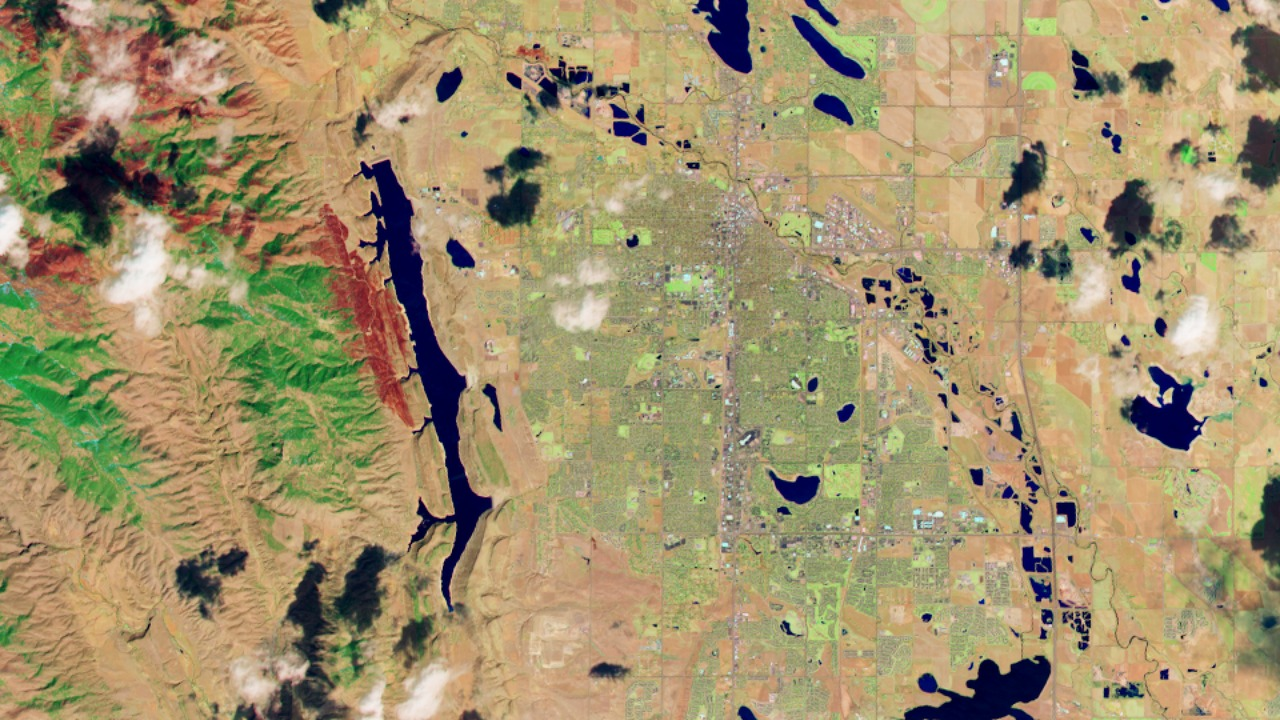
\includegraphics[width=.45\paperheight]{figures/landsatcolorado.jpg}
    \end{frame}
 
    \begin{frame}
        \frametitle{Landsat is a NASA satellite which captures images of the Earth.}
            \begin{figure}
            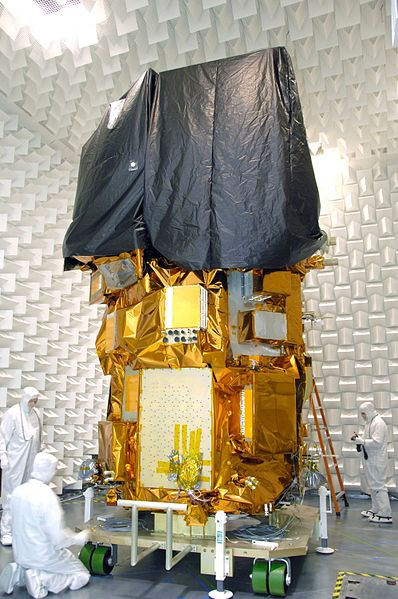
\includegraphics[width=.40\paperheight]{figures/groundlandsat.jpg}
            \caption{Landsat 8 from https://en.wikipedia.org/wiki/Landsat\_8}
            \end{figure}
    \end{frame}

    \begin{frame}
        \frametitle{The camera captures nine different wavelengths (3 visible, 3 infrared, panchromatic, and 2 for clouds)}
            \begin{figure}
            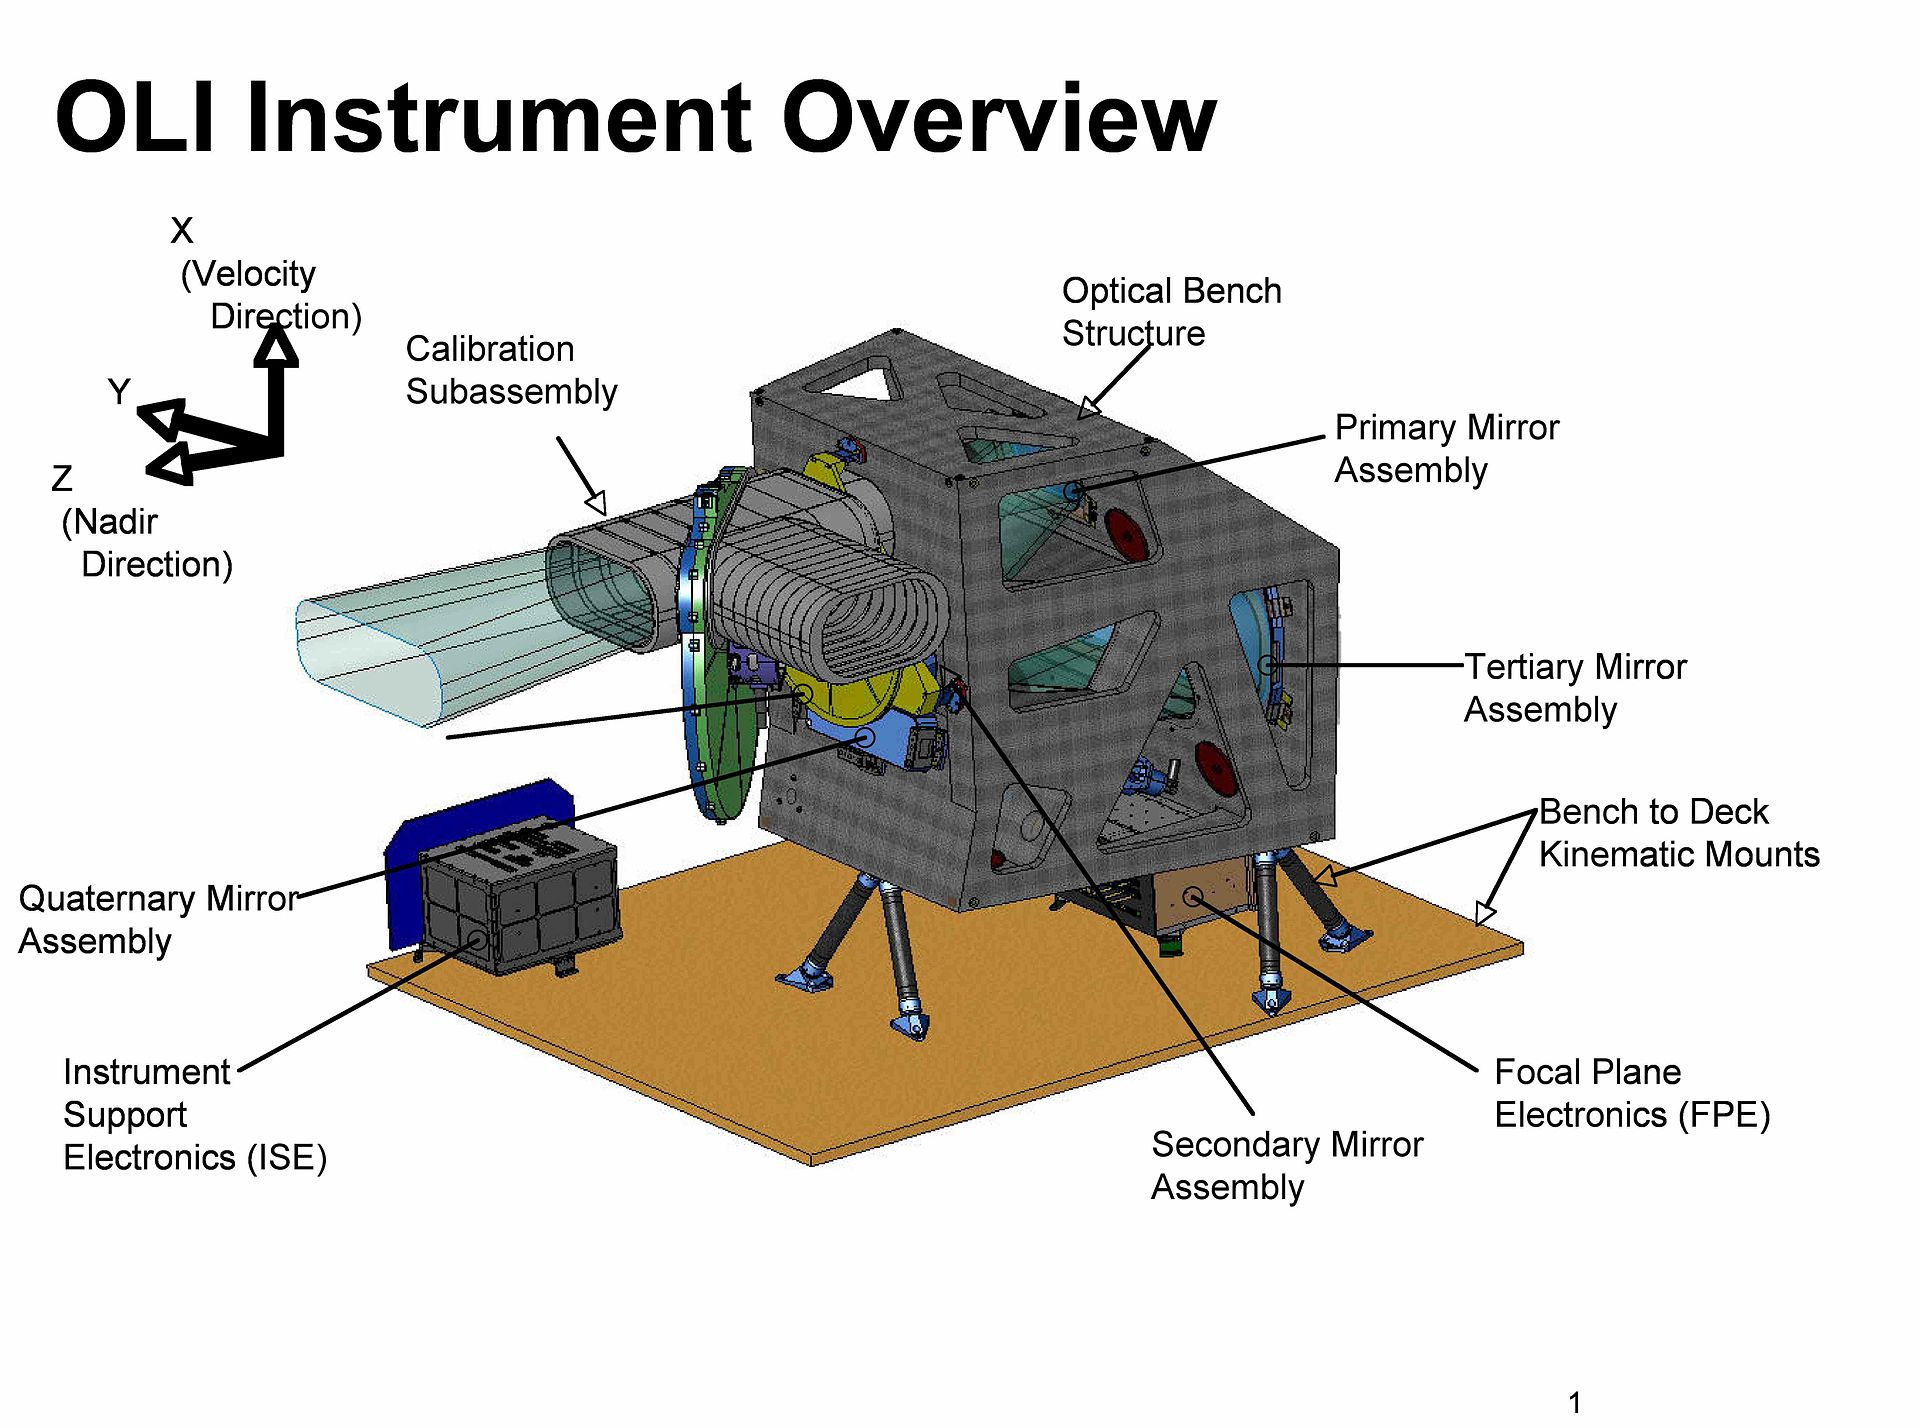
\includegraphics[width=.9\paperheight]{figures/landsatimager.jpg}
         \end{figure}
    \end{frame}

    \begin{frame}
        \frametitle{I created a Landsat Theater, a tool for downloading, processing, annotating landsat images}
            \begin{itemize}
                \item The multiple displays in the decision theater are used to visualize a place through time
                \item Landsat Theater downloads and processes imagery over a given location and annotates the images with metadata.
                \item The tool can display the images (working), or display the images with synchronized interactive zoom (in progress.. any of y'all know javascript?)
            \end{itemize}
         \end{figure}
    \end{frame}

    \begin{frame}
        \frametitle{For software design, I glued together a bunch of open source libraries..}
        \begin{description}
            \item[geopy] for converting cities or addresses to latitude and longitude
            \item[landsat-utils] for downloading and processing landsat data
            \item[PIL] (Python Image Library) for annotating landsat images with captions
            \item[tileup] for tiling
            \item[wx] for the searching, downloading, and processing GUI
            \item[leafletjs] for displaying images with synchronized interactive zooming (in progress)
        \end{description}
    \end{frame}
 
    \begin{frame}
        \frametitle{Landsat Theater could be extended...}
        \begin{itemize}
            \item The tool could clean up after itself better, it can easily fill up a hard drive..
            \item The tool lacks error handling and input sanitation.. 
            \item Landsat produces hyperspectral images, some wavelengths could be useful for comparing vegetation
            \item Finishing the interactive zoom would be great.
        \end{itemize}
    \end{frame}

    \begin{frame}
        \frametitle{Demo Time!}
            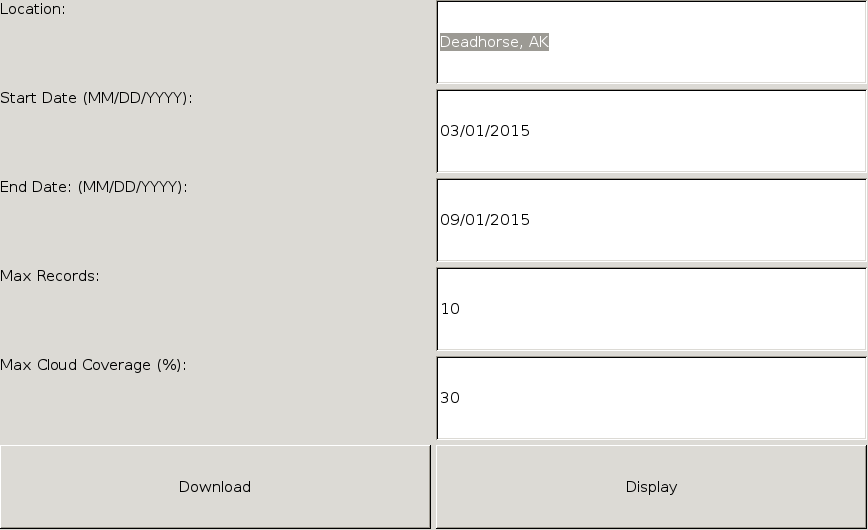
\includegraphics[width=3in]{figures/gui.png}
            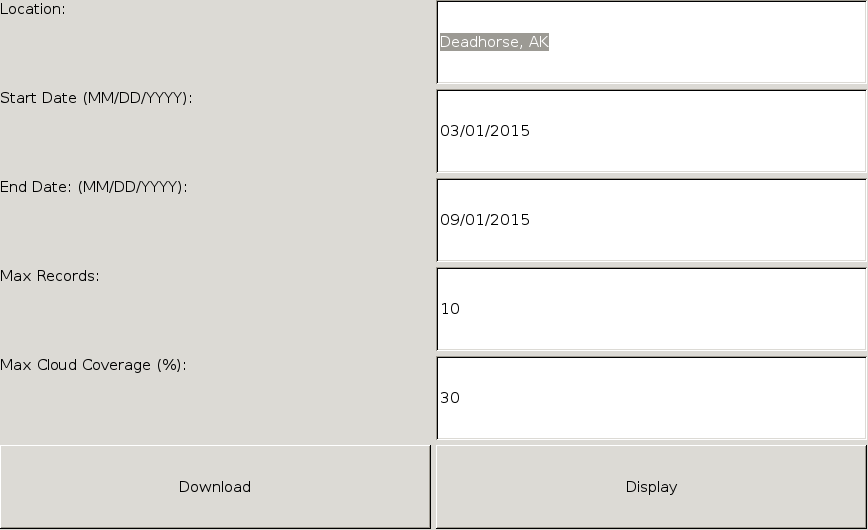
\includegraphics[width=3in]{figures/gui.png}
            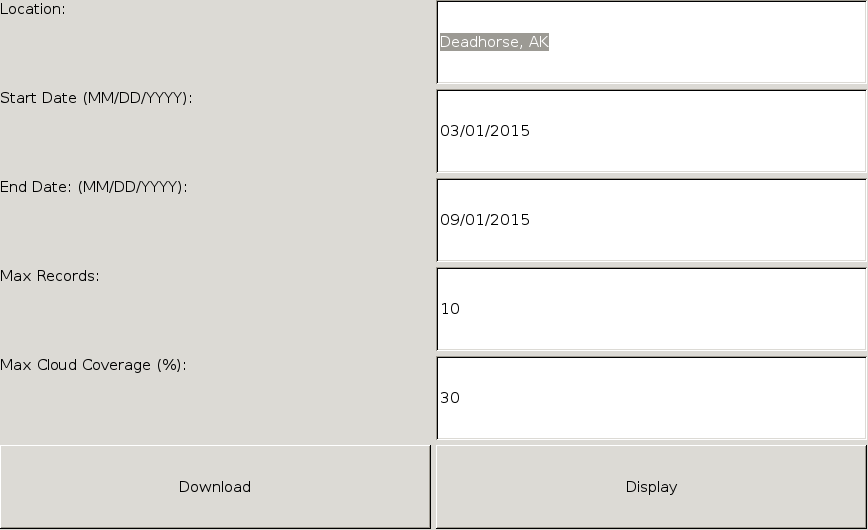
\includegraphics[width=3in]{figures/gui.png}
    \end{frame}
    
    \begin{frame}
        \frametitle{Questions?}
        My software is available under an open source license on GitHub:
        https://github.com/loxodes/fairbanks\_hackathon\_landsat\_viewer
    \end{frame}

\end{document}
